\documentclass[letterpaper,11pt]{article}
\oddsidemargin -1.0cm \textwidth 17.5cm

\usepackage[utf8]{inputenc}
\usepackage[activeacute,spanish, es-lcroman]{babel}
\decimalpoint
\usepackage{amsfonts,setspace}
\usepackage{amsmath}
\usepackage{amssymb, amsmath, amsthm}
\usepackage{comment}
\usepackage{float}
\usepackage{amssymb}
\usepackage{dsfont}
\usepackage{anysize}
\usepackage{multicol}
\usepackage{enumerate}
\usepackage{graphicx}
\usepackage[left=1.5cm,top=2cm,right=1.5cm, bottom=1.7cm]{geometry}
\setlength\headheight{1.5em} 
\usepackage{fancyhdr}
\usepackage{multicol}
\usepackage{hyperref}
\usepackage{wrapfig}
\usepackage{subcaption}
\usepackage{siunitx}
\usepackage{cancel}
\usepackage{mdwlist}
\usepackage{svg}
\pagestyle{fancy}
\fancyhf{}
\renewcommand{\labelenumi}{\normalsize\bfseries P\arabic{enumi}.}
\renewcommand{\labelenumii}{\normalsize\bfseries (\alph{enumii})}
\renewcommand{\labelenumiii}{\normalsize\bfseries \roman{enumiii})}


\begin{document}

\fancyhead[L]{\itshape{Facultad de Ciencias F\'isicas y Matem\'aticas}}
\fancyhead[R]{\itshape{Universidad de Chile}}

\begin{minipage}{11.5cm}
    \begin{flushleft}
        \hspace*{-0.6cm}\textbf{FI1000-6 Introducción a la Física Clásica}\\
        \hspace*{-0.6cm}\textbf{Profesora:} Paulina Lira\\
        \hspace*{-0.6cm}\textbf{Auxiliares:} Juan Cristóbal Castro \& Alejandro Silva\\
        \hspace*{-0.6cm}\textbf{Ayudantes:} Francisca Bórquez, Catalina Molina \& Erick Pérez\\
        
    \end{flushleft}
\end{minipage}

\begin{picture}(2,3)
    \put(366, 10){
\includegraphics[scale=0.9]{2020-1/Imágenes/logo/dfi-fcfm.pdf}}
\end{picture}

\begin{center}
	\LARGE\textbf{Auxiliar \#13}\\
	\Large{Estática de Sólido Rígido}
\end{center}

\vspace{-1cm}
\begin{enumerate}\setlength{\itemsep}{0.4cm}

\rfoot[]{pág. \thepage}

\item[]

\item Una barra homogénea de largo $L$ y masa $M$ reposa con un extremo fijo en un pivote en el suelo y el otro sostenido por una cuerda ideal, en donde los ángulos formados ($\alpha$, $\beta$) son conocidos.
    \begin{enumerate}
        \item Determine la tensión de la cuerda
        
        \item Determine la reacción en el punto de apoyo
    \end{enumerate}

    \begin{figure}[H]
      \centering
      \svgpath{../Imagenes/aux13}
      \includesvg[width=0.4\linewidth]{barra.svg}
    \end{figure}
    
\item Considere un lápiz de longitud $\ell$ y masa $m$ uniformemente distribuida colocado sobre una mesa horizontal de modo que el extremo inferior está sobre la mesa y el extremo superior reposa sobre el borde de un libro de alto $h$. El coeficiente de roce estático entre la mesa y el lápiz es $\mu$. Suponiendo que no hay roce entre el libro y el lápiz y que este se encuentra en equilibro.
    \begin{enumerate}
        \item Calcule la reacción normal que ejerce el libro sobre el lápiz y la reacción total (roce estático y reacción normal) ejercidos por el piso sobre el lápiz.
        
        \item Indique las condiciones que debe satisfacer la longitud $l$ del lápiz
        
        \item Determine el valor mínimo de $\mu$
    \end{enumerate}
    
    \begin{figure}[H]
      \centering
      \svgpath{../Imagenes/aux13}
      \includesvg[width=0.4\linewidth]{mesa.svg}
    \end{figure}

\newpage
\item Considere una semiesfera de radio $R$ de masa $M$ que se encuentra sobre una superficie horizontal y apoyada contra una pared tal como se muestra en la figura adjunta. El centro de masas de una semiesfera homogénea queda sobre el eje de simetría y a una distancia ${b} = 3 R / 8$ de la base. Suponga que, entre la semiesfera y el suelo el coeficiente de roce estático es $\mu = 3 / 16$, mientras que entre la pared y la semiesfera el roce es nulo.
    \begin{enumerate}
        \item Realice un diagrama de cuerpo libre para la semiesfera.
        \item Encuentre la magnitud y dirección del torque, respecto al punto de apoyo $P$, ejercido por la fuerza de gravedad cuando la semiesfera está ladeada en un ángulo $\beta$.
        \item Encuentre la fuerza de roce entre la semi-esfera y el suelo
        \item Encuentre el ángulo de inclinación mínimo $\beta_{min}$ posible para que la semiesfera no resbale.
    \end{enumerate}
    
    \begin{figure}[H]
        \centering
        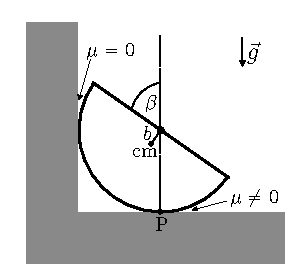
\includegraphics[width=0.35\linewidth]{2020-1/Imágenes/aux Extra-C2/semiesfera-torque.pdf}
    \end{figure}


% Para imágenes vectoriales -> el texto tiene que estar en LaTeX
% \begin{figure}[htbp]
%   \centering
%   \svgpath{../Imagenes/ejercicios}  -> .. irse pa'trás 
%   \includesvg{ej5.svg}
% \end{figure}

\end{enumerate}
\end{document}
